\documentclass[11pt,a4paper]{article}

% ---- Core math & symbols ----
\usepackage{amsmath,amssymb,amsthm,amsfonts,mathtools}

% ---- Page geometry & typography ----
\usepackage[a4paper,margin=1.1in]{geometry}
\usepackage[T1]{fontenc}
\IfFileExists{lmodern.sty}{\usepackage{lmodern}\usepackage{microtype}}{}
\usepackage{setspace}
\setstretch{1.08}

% ---- Graphics & diagrams ----
\usepackage{tikz}
\usetikzlibrary{arrows.meta, positioning, shapes.geometric, fit, calc, shadows.blur, backgrounds, decorations.pathreplacing}

% ---- Aesthetics ----
\usepackage{xcolor}
\definecolor{primeblue}{RGB}{28,60,110}
\definecolor{primeaccent}{RGB}{180,60,60}
\definecolor{softgray}{RGB}{240,240,245}
\definecolor{trainerblue}{RGB}{200,220,245}
\definecolor{inferencegreen}{RGB}{210,235,215}
\definecolor{orchgray}{RGB}{225,225,230}
\definecolor{kvyellow}{RGB}{252,242,205}

% ---- Epigraphs, quotes, lists ----
\usepackage{epigraph}
\setlength{\epigraphwidth}{0.62\textwidth}
\renewcommand{\epigraphflush}{flushright}
\renewcommand{\textflush}{flushright}
\renewcommand{\epigraphrule}{0pt}
\usepackage{enumitem}
\usepackage{booktabs}
\setlist{itemsep=2pt, topsep=4pt}

% ---- Cross-references & links ----
\usepackage[colorlinks=true,linkcolor=primeblue,citecolor=primeblue,urlcolor=primeblue]{hyperref}

% ---- Theorem-like environments ----
\theoremstyle{definition}
\newtheorem{definition}{Definition}[section]
\newtheorem{remark}[definition]{Remark}
\newtheorem{example}[definition]{Example}

\theoremstyle{plain}
\newtheorem{proposition}[definition]{Proposition}

% ---- Custom macros ----
\newcommand{\R}{\mathbb{R}}
\newcommand{\E}{\mathbb{E}}
\newcommand{\KL}{\mathrm{KL}}
\newcommand{\policy}{\pi_\theta}
\newcommand{\oldpolicy}{\pi_{\theta_{\text{old}}}}
\newcommand{\refpolicy}{\pi_{\text{ref}}}

% ---- Title ----
\title{\vspace{-1.5em}\textbf{Scaling Agentic Reinforcement Learning} \\[0.4em]
  {\large Lecture 10}}
\date{}

\begin{document}
\maketitle

\begin{abstract}
\noindent These notes accompany a lecture on the scaling of reinforcement learning (RL) for large language models, with an emphasis on the agentic regime. We trace the algorithmic lineage from RLHF through RLVR to the emerging discipline of long-horizon agentic RL, and we examine in detail the infrastructural machinery required to train a frontier Mixture-of-Experts model at the scale of Intellect-3. Particular attention is paid to the asymmetry between training and inference, the art of asynchronous rollout orchestration, and the subtle algorithmic price one pays for off-policy data: importance sampling, PPO clipping, and KL regularization. We close with a survey of the inference-side optimizations --- expert parallelism, prefill/decode disaggregation, and low-bit quantization --- that make agentic RL tractable at all.
\end{abstract}

\tableofcontents
\vspace{1em}
\hrule
\vspace{1em}

% =====================================================================
\section{Prologue: From Passive Knowledge to Active Experience}
% =====================================================================

\epigraph{``What I cannot create, I do not understand.''}{--- Richard Feynman}

The recent efflorescence of large language models has been driven almost entirely by \emph{pretraining}: the ingestion, at industrial scale, of the textual record of humanity, compressed via next-token prediction into a dense parametric representation of the world. A model so trained is a prodigious scholar --- it has read, in a manner of speaking, everything --- but it has \emph{done} nothing. It is the educated student of Borges' library, fluent in every volume yet with no body to act and no goals to pursue.

Reinforcement learning introduces the missing ingredient. Where pretraining is passive absorption, RL is \emph{active learning from the world via experience}. An agent proposes, the environment disposes, and a reward signal --- parsimonious, sometimes delayed, occasionally capricious --- teaches the agent to refine its policy. The transition we are witnessing, then, is a transition from models that \emph{know} to models that \emph{do}.

\begin{definition}[Policy]
A \emph{policy} $\pi_\theta(y \mid x)$ is a (typically stochastic) mapping from states $x$ to distributions over actions $y$, parameterized by $\theta$. In the LLM setting, $x$ is a prompt (possibly augmented by history and tool outputs) and $y$ is a token or token sequence. The policy is called \emph{on-policy} when actions used for optimization are drawn from the same distribution that is being updated, and \emph{off-policy} otherwise.
\end{definition}

% =====================================================================
\section{The Arc of RL Scaling, 2023--2026}
% =====================================================================

A striking empirical observation animates this course: every major recent inflection in AI capability has been underwritten by a particular flavor of reinforcement learning, scaled to unprecedented size. The genealogy is clean enough to draw on a single axis.

\begin{center}
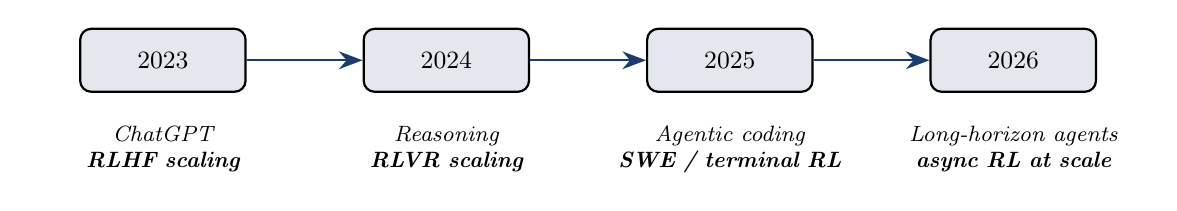
\begin{tikzpicture}[
  every node/.style={font=\small},
  year/.style={draw, rounded corners, fill=primeblue!12, minimum width=2.1cm, minimum height=0.8cm, thick},
  caption/.style={text width=3.2cm, align=center, font=\footnotesize\itshape},
  arr/.style={-{Stealth[length=3mm]}, thick, primeblue}
]
  \node[year] (a) at (0,0) {2023};
  \node[year] (b) at (3.6,0) {2024};
  \node[year] (c) at (7.2,0) {2025};
  \node[year] (d) at (10.8,0) {2026};

  \draw[arr] (a) -- (b);
  \draw[arr] (b) -- (c);
  \draw[arr] (c) -- (d);

  \node[caption, below=0.3cm of a] {ChatGPT \\ \textbf{RLHF scaling}};
  \node[caption, below=0.3cm of b] {Reasoning \\ \textbf{RLVR scaling}};
  \node[caption, below=0.3cm of c] {Agentic coding \\ \textbf{SWE / terminal RL}};
  \node[caption, below=0.3cm of d] {Long-horizon agents \\ \textbf{async RL at scale}};
\end{tikzpicture}
\end{center}

\noindent The progression is not accidental. Each rung of the ladder transforms what counts as a \emph{reward}, and what counts as a reward determines what can be learned.

\begin{itemize}
  \item \textbf{2023 --- RLHF.} Reinforcement learning from human feedback transformed raw base models into interlocutors. The reward was a learned proxy for human preference. The breakthrough was \emph{alignment} with conversational norms.
  \item \textbf{2024 --- RLVR.} Reinforcement learning from \emph{verifiable} rewards --- unit tests, known mathematical answers, compiler exit codes --- freed training from the bottleneck of human labelers. Reasoning models, with their long internal chains of thought, are the direct fruit of this shift.
  \item \textbf{2025 --- Agentic coding.} The reward signal moved into the terminal itself: did the pull request pass CI? Did the script run? The model began to \emph{inhabit} an environment rather than merely generate text.
  \item \textbf{2026 --- Long-horizon agents.} The frontier. Tasks spanning hours or days, sparse terminal rewards, multi-stage planning. The infrastructural and algorithmic demands here are qualitatively different, and much of what follows in these notes is aimed squarely at making this regime feasible.
\end{itemize}

% =====================================================================
\section{Intellect-3: Model, Scale, and Training Stack}
% =====================================================================

Much of the concrete discussion that follows is grounded in the training of \textbf{Intellect-3}, a 100-billion-parameter Mixture-of-Experts (MoE) model co-developed at Prime Intellect. Intellect-3 achieves state-of-the-art results for its size class on the ADM (algebraic deduction), QED, and SWE (software engineering) benchmark suites across several contest years.

\begin{remark}[Why MoE]
In a \emph{dense} model, every parameter is activated for every input, and the model's capacity is bounded by what can be economically trained and served at that density. A Mixture-of-Experts architecture routes each token to a sparse subset of specialized expert subnetworks, decoupling total parameter count from per-token compute. The cost, as we shall see in Section~\ref{sec:inference-infra}, is paid in routing complexity, load-balancing, and the delicate art of serving large expert populations under expert parallelism.
\end{remark}

The model was post-trained on a cluster of more than 512 H200 GPUs. The sheer hardware footprint is worth pausing on: the inefficiencies we shall soon enumerate are not rounding errors. A 50\% idling of a 512-GPU cluster is a substantive economic and scientific loss, and much of the engineering ingenuity of the field is directed at recovering those wasted cycles.

% =====================================================================
\section{Reinforcement Learning from Verifiable Rewards}
% =====================================================================

We now sharpen our algorithmic vocabulary. RLVR is the workhorse of contemporary reasoning-model training, and its mechanics repay careful study.

\subsection{Verifiable Problems and Group-Relative Advantage}

\begin{definition}[Verifiable Problem]
A problem is \emph{verifiable} if there exists a computable grader $V: \mathcal{Y} \to \{0,1\}$ (or, more generally, to $[0,1]$) that evaluates any candidate solution $y$ against a ground truth. Typical examples: mathematical problems with known answers, coding problems equipped with unit tests, puzzles with checkable solutions.
\end{definition}

\begin{remark}[A note on GRPO and the broader family]
The group-relative scheme introduced below is the defining feature of
\emph{Group Relative Policy Optimization} (GRPO), and it is worth stating
plainly that GRPO is only one member of a large family of policy-gradient
methods. Classical REINFORCE uses a single sampled return with no baseline;
actor--critic and standard PPO learn a separate value network to estimate the
baseline; methods such as RLOO construct a leave-one-out baseline from a group
of samples. GRPO's distinguishing move is to dispense with the learned critic
entirely and use the \emph{group mean} as the baseline --- cheaper to
implement and one fewer network to train and stabilize. None of these is
canonically ``correct''; each trades off variance, bias, and engineering
overhead differently, and the right choice remains an active research
question. We foreground GRPO here not because it is provably superior but
because the field has, over the past year, largely converged on it as the
default for RLVR at scale; treating it as our running example keeps these
notes aligned with current practice while the reader should bear in mind that
the surrounding infrastructure --- asynchrony, importance sampling, clipping
--- is largely agnostic to which advantage estimator sits at its center.
\end{remark}

% ---------------------------------------------------------------------

For each prompt $x$ in a training batch, the model generates a \emph{group} of $G$ independent completions $\{y^{(1)}, \ldots, y^{(G)}\}$ (a common choice is $G=16$). Each is scored by the verifier, yielding rewards $r^{(i)} = V(y^{(i)}) \in \{0,1\}$. The \emph{group-relative advantage} of the $i$-th completion is
\begin{equation}
  \hat{A}^{(i)} \;=\; r^{(i)} - \frac{1}{G}\sum_{j=1}^{G} r^{(j)}.
\end{equation}
This subtraction of the group mean is not a mere variance-reduction trick: it shifts the learning signal from \emph{absolute} correctness to \emph{relative} improvement within a shared context. A completion that succeeds where the group fails receives a large positive signal; one that fails where the group succeeds receives a large negative one. The model is pressed to discover and reinforce the trajectories --- the reasoning chains --- that outperform its own average attempt.

\begin{example}[Group-relative advantage, by hand]
Take a small group, $G=4$, and a binary verifier. The model produces four
completions for one prompt and the verifier returns
\[
  r^{(1)}=1,\quad r^{(2)}=0,\quad r^{(3)}=1,\quad r^{(4)}=0.
\]
The group baseline is the mean reward,
\[
  \bar{r} = \tfrac{1}{4}(1+0+1+0) = 0.5,
\]
and the group-relative advantages are
\[
  \hat{A}^{(1)} = 1-0.5 = +0.5,\quad
  \hat{A}^{(2)} = 0-0.5 = -0.5,\quad
  \hat{A}^{(3)} = +0.5,\quad
  \hat{A}^{(4)} = -0.5.
\]
Two observations. First, the advantages sum to zero by construction
($\sum_i \hat{A}^{(i)} = \sum_i r^{(i)} - G\bar{r} = 0$); the update reinforces
the winners exactly as much as it suppresses the losers. Second, the
\emph{magnitude} of the signal depends on how split the group is. If instead
all four had succeeded ($\bar r = 1$), every advantage would be $0$ and the
prompt would contribute \emph{no} gradient at all --- a solved problem teaches
the model nothing. The sharpest learning signal comes from prompts the model
gets right about half the time, where $\bar r \approx 0.5$ and $|\hat A|$ is
maximal. This is why curricula drift toward problems of intermediate
difficulty: they carry the most information per rollout.
\end{example}

% ---------------------------------------------------------------------

\subsection{Chain-of-Thought as an Emergent Consequence}

It is worth dwelling on what is, and is not, being rewarded. The verifier sees only the final answer. Yet the model, given room to produce a long scratchpad before committing to that answer, reliably develops elaborate chains of thought during RLVR training. The explanation is statistical: reasoning \emph{works}. Trajectories that reason carefully are more likely to produce verified answers, and therefore receive positive advantage, and therefore have their probability mass increased. Chain-of-thought is not designed in; it is selected for.

\subsection{The Policy Gradient and PPO Clipping}

The core policy gradient objective is to maximize expected reward:
\begin{equation}
  J(\theta) \;=\; \E_{x \sim \mathcal{D},\, y \sim \pi_\theta(\cdot \mid x)}\bigl[R(y)\bigr],
  \qquad
  \nabla_\theta J(\theta) \;\approx\; \E\bigl[\hat{A}\,\nabla_\theta \log \pi_\theta(y \mid x)\bigr].
\end{equation}
Left to its own devices, this objective can take ruinously large steps: a single batch of high-advantage trajectories can deform the policy so violently that subsequent rollouts collapse to degenerate modes. Proximal Policy Optimization (PPO) addresses this by clipping the probability ratio
\begin{equation}
  r(\theta) \;=\; \frac{\pi_\theta(y \mid x)}{\pi_{\theta_{\text{old}}}(y \mid x)},
\end{equation}
yielding the clipped surrogate objective
\begin{equation}
  L^{\text{CLIP}}(\theta) \;=\; \E\!\left[\,\min\!\Bigl(r(\theta)\,\hat{A},\;\operatorname{clip}\!\bigl(r(\theta),\,1-\varepsilon,\,1+\varepsilon\bigr)\,\hat{A}\Bigr)\,\right].
\end{equation}

\begin{example}[What the clip actually does to one sample]
Fix $\varepsilon = 0.2$, so the clip range is $[0.8,\,1.2]$. Consider four
samples with assorted ratios $r(\theta)=\policy/\oldpolicy$ and advantages
$\hat A$. The PPO term keeps the \emph{smaller} of the unclipped and clipped
products:
\begin{center}
\renewcommand{\arraystretch}{1.3}
\begin{tabular}{@{}ccccc@{}}
\toprule
$r(\theta)$ & $\hat A$ & $r\,\hat A$ & $\operatorname{clip}(r)\,\hat A$ & $\min(\cdot)$ used \\
\midrule
$1.5$ & $+1$ & $+1.5$ & $+1.2$ & $\mathbf{+1.2}$ \\
$1.5$ & $-1$ & $-1.5$ & $-1.2$ & $\mathbf{-1.5}$ \\
$0.5$ & $+1$ & $+0.5$ & $+0.8$ & $\mathbf{+0.5}$ \\
$0.5$ & $-1$ & $-0.5$ & $-0.8$ & $\mathbf{-0.8}$ \\
\bottomrule
\end{tabular}
\end{center}
Read the asymmetry off the bold column. When the advantage is
\emph{positive} (row 1), the clip refuses to let an over-eager ratio
($r=1.5$) push harder than $1.2$: gains are capped. When the advantage is
\emph{negative} (row 2), the unclipped $-1.5$ is smaller than $-1.2$, so the
$\min$ keeps the full $-1.5$: the penalty is \emph{not} capped. PPO is
deliberately lenient about pushing probability \emph{down} on bad trajectories
and strict about pushing it \emph{up} on good ones. That asymmetry is the
trust region in action --- it is far safer to abandon a trajectory than to
over-commit to one.
\end{example}

% ---------------------------------------------------------------------

The clip confines each update to a \emph{trust region} around the old policy. Beyond the clip, one typically layers a Kullback--Leibler regularizer against a reference policy $\pi_{\text{ref}}$ (often the pre-RL checkpoint) to anchor the model against policy drift:
\begin{equation}
  L^{\text{TOTAL}}(\theta) \;=\; L^{\text{CLIP}}(\theta) \;-\; \beta\, \KL\!\bigl(\pi_\theta \,\big\|\, \refpolicy\bigr).
  \label{eq:total-objective}
\end{equation}
Equation~\eqref{eq:total-objective} is, to a first approximation, the objective that trains a modern reasoning model. Everything else in this document is either upstream (how we generate the data) or downstream (how we make the gradient step efficient on a cluster).

% =====================================================================
\section{The End-to-End RLVR Loop}
% =====================================================================

\begin{center}
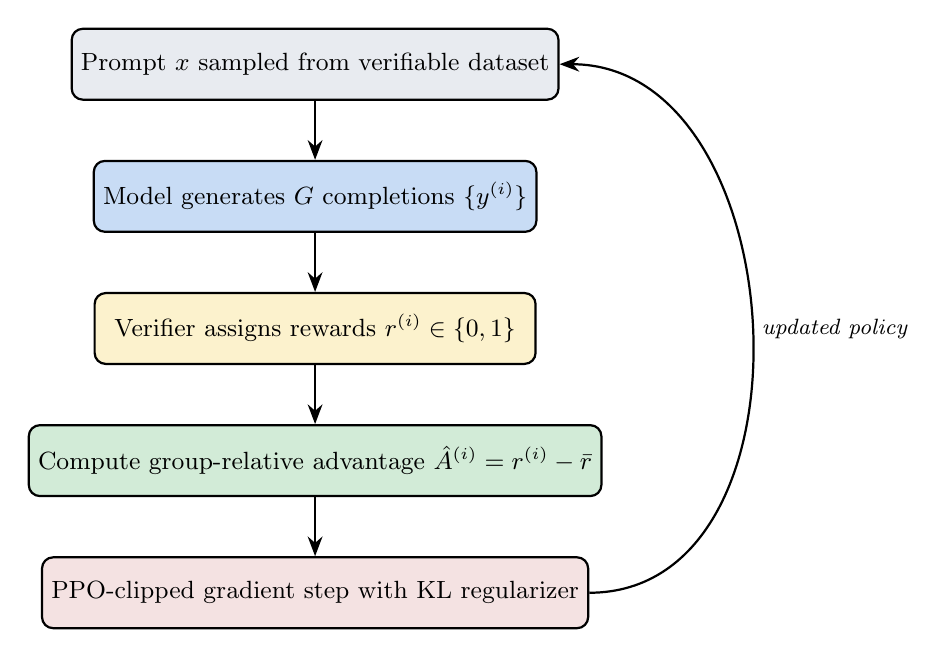
\begin{tikzpicture}[
  node distance=0.75cm,
  box/.style={draw, rounded corners, thick, minimum width=5.6cm, minimum height=0.9cm, align=center, font=\small},
  arr/.style={-{Stealth[length=2.5mm]}, thick}
]
  \node[box, fill=primeblue!10] (p) {Prompt $x$ sampled from verifiable dataset};
  \node[box, fill=trainerblue, below=of p] (g) {Model generates $G$ completions $\{y^{(i)}\}$};
  \node[box, fill=kvyellow, below=of g] (v) {Verifier assigns rewards $r^{(i)} \in \{0,1\}$};
  \node[box, fill=inferencegreen, below=of v] (a) {Compute group-relative advantage $\hat{A}^{(i)} = r^{(i)} - \bar{r}$};
  \node[box, fill=primeaccent!15, below=of a] (u) {PPO-clipped gradient step with KL regularizer};

  \draw[arr] (p) -- (g);
  \draw[arr] (g) -- (v);
  \draw[arr] (v) -- (a);
  \draw[arr] (a) -- (u);
  \draw[arr] (u.east) .. controls +(3,0) and +(3,0) .. node[right, font=\footnotesize\itshape]{updated policy} (p.east);
\end{tikzpicture}
\end{center}

% =====================================================================
\section{Training and Inference: Two Very Different Animals}
% =====================================================================

An RL system is not a single program; it is two programs in dialogue. Understanding why they cannot easily share hardware is the key to understanding everything that follows.

\subsection{The Training Workflow}

Training is a synchronous, gradient-producing process. For models of serious scale, weights, gradients, and optimizer states are sharded across the cluster via \textbf{Fully Sharded Data Parallelism} (FSDP/FSDP2), with gradients synchronized by \texttt{AllReduce}. Context and tensor parallelism layer on top for models whose individual layers exceed single-device memory.

\begin{center}
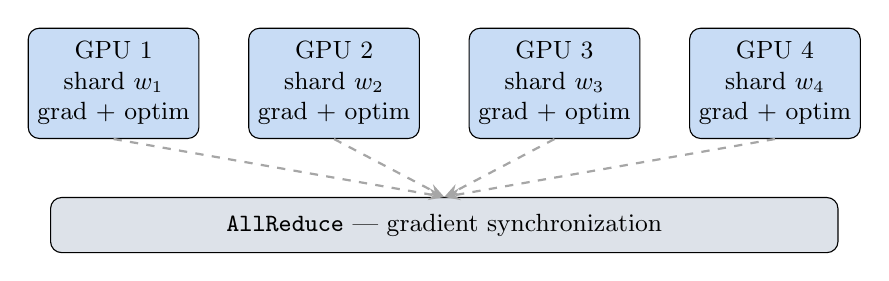
\begin{tikzpicture}[
  gpu/.style={draw, rounded corners, fill=trainerblue, minimum width=2cm, minimum height=1.4cm, align=center, font=\small},
  arr/.style={-{Stealth[length=2mm]}, thick, dashed, gray!70}
]
  \node[gpu] (g1) at (0,0)   {GPU 1 \\ shard $w_1$ \\ grad + optim};
  \node[gpu] (g2) at (2.8,0) {GPU 2 \\ shard $w_2$ \\ grad + optim};
  \node[gpu] (g3) at (5.6,0) {GPU 3 \\ shard $w_3$ \\ grad + optim};
  \node[gpu] (g4) at (8.4,0) {GPU 4 \\ shard $w_4$ \\ grad + optim};

  \node[draw, rounded corners, fill=primeblue!15, minimum width=10cm, minimum height=0.7cm] (ar) at (4.2,-1.8) {\small \texttt{AllReduce} --- gradient synchronization};

  \draw[arr] (g1.south) -- (ar.north);
  \draw[arr] (g2.south) -- (ar.north);
  \draw[arr] (g3.south) -- (ar.north);
  \draw[arr] (g4.south) -- (ar.north);
\end{tikzpicture}
\end{center}

\subsection{The Inference Workflow}

Inference, by contrast, is autoregressive: tokens emerge one at a time, each conditioned on its predecessors. The relevant optimizations are not about gradient synchronization but about managing the growing key-value cache and about keeping the GPU fed with work.

\begin{description}[style=nextline, leftmargin=0.6cm, itemsep=4pt]
  \item[Paged attention.] The KV cache is allocated in fixed-size blocks, analogous to pages in a virtual-memory system. This eliminates the fragmentation that otherwise plagues variable-length sequences.
  \item[Continuous batching.] Rather than wait for the slowest sequence in a batch to finish, completed slots are immediately refilled with new requests. Tokens stream out as they become ready.
  \item[Tensor parallelism (TP).] Individual weight matrices are sharded across devices so that each forward pass engages the whole node in concert, reducing latency at the cost of communication.
\end{description}

\begin{center}
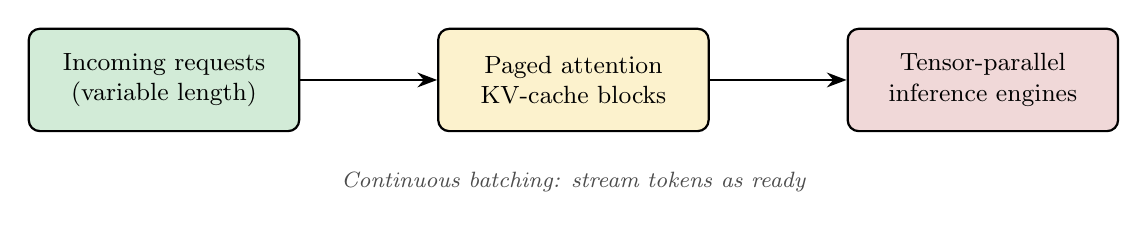
\begin{tikzpicture}[
  box/.style={draw, rounded corners, thick, minimum height=1.3cm, align=center, font=\small},
  arr/.style={-{Stealth[length=2.5mm]}, thick}
]
  \node[box, fill=inferencegreen, text width=3.2cm] (req) at (0,0) {Incoming requests \\ (variable length)};
  \node[box, fill=kvyellow, text width=3.2cm] (kv) at (5.2,0) {Paged attention \\ KV-cache blocks};
  \node[box, fill=primeaccent!20, text width=3.2cm] (tp) at (10.4,0) {Tensor-parallel \\ inference engines};

  \draw[arr] (req) -- (kv);
  \draw[arr] (kv) -- (tp);

  \node[font=\footnotesize\itshape, gray!60!black] at (5.2,-1.3) {Continuous batching: stream tokens as ready};
\end{tikzpicture}
\end{center}

\subsection{The Fundamental Incompatibility}

Training wants FSDP; inference wants TP. Training benefits from large batches and stable layouts; inference benefits from continuous batching and paged memory. The software stacks are different (e.g.\ FSDP2 vs.\ vLLM/TensorRT-LLM). The operator kernels are different. Even when the \emph{mathematical} model is identical, its two instantiations are, in practice, two distinct programs that cannot easily time-share a GPU.

\begin{remark}[The floating-point footnote]\label{rem:fp}
Even when training and inference load \emph{the same weights on the same hardware}, their output distributions will differ. The reason is prosaic but consequential: matrix multiplications involving tensors of different shapes dispatch to different kernels with different reduction orders, and floating-point addition is not associative. The resulting numerical drift, small on any single token, compounds over long sequences and is sufficient to make nominally ``on-policy'' data mildly off-policy. This is not a bug to paper over; it must be corrected algorithmically, via the machinery of Section~\ref{sec:async-corrections}.
\end{remark}

% =====================================================================
\section{Na\"ive RL Infrastructure and Its Discontents}
% =====================================================================

The simplest way to reconcile training and inference on one cluster is to \emph{alternate}: let the GPUs serve as inference engines, generate a batch of rollouts, then reconfigure the parallelism, reload the weights in training layout, and take a gradient step.

\begin{center}
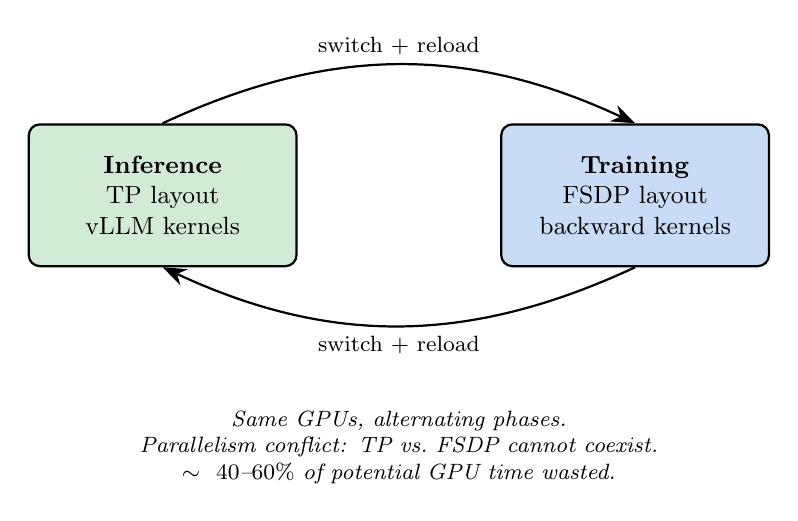
\begin{tikzpicture}[
  phase/.style={draw, rounded corners, thick, minimum width=3.4cm, minimum height=1.8cm, align=center, font=\small},
  arr/.style={-{Stealth[length=3mm]}, thick}
]
  \node[phase, fill=inferencegreen] (inf) at (0,0) {\textbf{Inference}\\TP layout \\ vLLM kernels};
  \node[phase, fill=trainerblue] (tr) at (6,0) {\textbf{Training}\\FSDP layout \\ backward kernels};

  \draw[arr, bend left=25] (inf.north) to node[above, font=\footnotesize] {switch + reload} (tr.north);
  \draw[arr, bend left=25] (tr.south) to node[below, font=\footnotesize] {switch + reload} (inf.south);

  \node[align=center, font=\footnotesize\itshape, text width=8cm] at (3,-3.2) {Same GPUs, alternating phases. \\ Parallelism conflict: TP vs.\ FSDP cannot coexist. \\ $\sim\!40\text{--}60\%$ of potential GPU time wasted.};
\end{tikzpicture}
\end{center}

The arithmetic is grim. Between every optimizer step, the system pays in full for two context switches: one to tear down the training configuration and stand up the inference server, and one to reverse the transformation. When measured against the cost of a 512-GPU cluster, this idle time is not a quibble. It is, fundamentally, a software architecture problem masquerading as a hardware problem.

% =====================================================================
\section{Asynchronous Infrastructure: The Disaggregated Design}
% =====================================================================

The decisive improvement is \emph{disaggregation}: we stop asking one pool of GPUs to do both jobs. Instead, we partition the cluster permanently --- say, half for inference, half for training --- and let the two halves run independently, exchanging data and weights as they go.

\subsection{The Architectural Picture}

\begin{center}
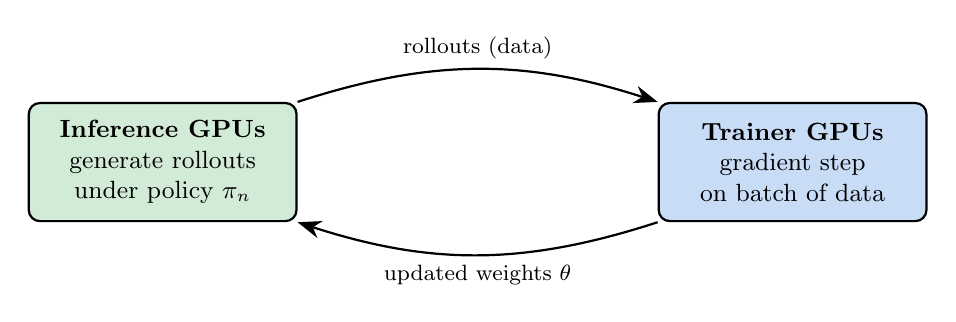
\begin{tikzpicture}[
  box/.style={draw, rounded corners, thick, minimum width=3.4cm, minimum height=1.5cm, align=center, font=\small},
  arr/.style={-{Stealth[length=3mm]}, thick}
]
  \node[box, fill=inferencegreen] (inf) at (0,0) {\textbf{Inference GPUs}\\generate rollouts\\under policy $\pi_n$};
  \node[box, fill=trainerblue] (tr) at (8,0) {\textbf{Trainer GPUs}\\gradient step\\on batch of data};

  \draw[arr, bend left=18] (inf.north east) to node[above, font=\footnotesize] {rollouts (data)} (tr.north west);
  \draw[arr, bend left=18] (tr.south west) to node[below, font=\footnotesize] {updated weights $\theta$} (inf.south east);
\end{tikzpicture}
\end{center}

Both halves run at full speed at all times. The trainer never waits on inference; inference never waits on the trainer. The cluster is constantly busy.

\subsection{The Price of Asynchrony: Stale Gradients}

This efficiency has a subtle cost. By the time a batch of rollouts, generated under policy $\pi_{n-1}$, reaches the trainer, the trainer is already updating a policy $\pi_n$ (or $\pi_{n-k}$ for a pipeline of depth $k$). The data is \emph{off-policy} with respect to the policy being optimized. Na\"ively applying the policy gradient to such data can cause the algorithm to drift or collapse.

\begin{center}
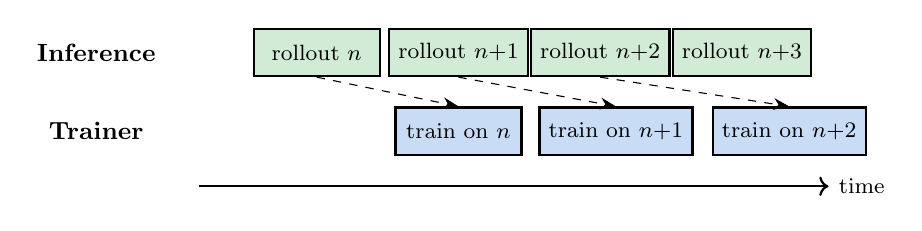
\begin{tikzpicture}[
  rect/.style={draw, thick, minimum width=1.6cm, minimum height=0.6cm, font=\footnotesize, align=center},
  lbl/.style={font=\small\bfseries}
]
  \node[lbl] at (-2.8, 1) {Inference};
  \node[lbl] at (-2.8, 0) {Trainer};

  \node[rect, fill=inferencegreen] (i1) at (0,1) {rollout $n$};
  \node[rect, fill=inferencegreen] (i2) at (1.8,1) {rollout $n{+}1$};
  \node[rect, fill=inferencegreen] (i3) at (3.6,1) {rollout $n{+}2$};
  \node[rect, fill=inferencegreen] (i4) at (5.4,1) {rollout $n{+}3$};

  \node[rect, fill=trainerblue] (t1) at (1.8,0) {train on $n$};
  \node[rect, fill=trainerblue] (t2) at (3.8,0) {train on $n{+}1$};
  \node[rect, fill=trainerblue] (t3) at (6.0,0) {train on $n{+}2$};

  \draw[-{Stealth[length=2mm]}, dashed] (i1.south) -- (t1.north);
  \draw[-{Stealth[length=2mm]}, dashed] (i2.south) -- (t2.north);
  \draw[-{Stealth[length=2mm]}, dashed] (i3.south) -- (t3.north);

  \draw[->, thick] (-1.5, -0.7) -- (6.5, -0.7) node[right, font=\footnotesize] {time};
\end{tikzpicture}
\end{center}

\subsection{Why Staleness Explodes: A Closer Look}

The notes have so far described stale data as merely ``off-policy.'' It is
worth seeing precisely how a small per-step disagreement compounds into a
catastrophe, because the failure is not gradual decay but a variance
explosion.

The policy gradient is an expectation taken \emph{under the current policy}:
\begin{equation}
  \nabla_\theta J(\theta)
  \;=\; \E_{y \sim \policy}\!\bigl[\hat A(y)\,\nabla_\theta \log \policy(y\mid x)\bigr].
\end{equation}
A stale rollout draws $y$ from $\oldpolicy$ instead. To remain unbiased we
must reweight each trajectory by its importance weight. For an
autoregressive policy over a length-$T$ sequence, that weight is a
\emph{product} of per-token ratios:
\begin{equation}
  w \;=\; \frac{\policy(y\mid x)}{\oldpolicy(y\mid x)}
        \;=\; \prod_{t=1}^{T}
              \frac{\policy(y_t \mid y_{<t},x)}{\oldpolicy(y_t \mid y_{<t},x)}.
  \label{eq:isw-product}
\end{equation}
The product is the whole problem. Even if every per-token ratio sits
innocuously near $1$, multiplying $T$ of them lets the total wander far from
$1$, and it does so with variance that grows with both the sequence length
$T$ and the staleness $k$ (how many optimizer steps separate $\oldpolicy$
from $\policy$). Importance sampling removes the \emph{bias} but pays for it
in \emph{variance}, and it is the variance that destabilizes training.

\begin{example}[A 1\% drift over a long sequence]
Suppose the trainer has moved just slightly ahead of the inference weights,
so that on average each per-token ratio is
$\policy/\oldpolicy \approx 1.01$ --- a one-percent disagreement, the kind of
thing the floating-point footnote of Remark~4.99 alone could produce.
Over a short $T=50$ token answer,
\[
  w \approx 1.01^{50} \approx 1.64,
\]
already a $64\%$ over-weighting. Over a long agentic rollout of
$T = 2000$ tokens,
\[
  w \approx 1.01^{2000} \approx 4.4 \times 10^{8}.
\]
A single trajectory now carries a weight of several hundred million. Dropped
unclipped into a batch, it annihilates every other sample's contribution: the
``average'' gradient becomes that one trajectory's gradient, pointing in an
essentially arbitrary direction. The next rollouts are drawn even further
off-distribution, and the run collapses. This is the precise mechanism behind
the warning that na\"ive off-policy updates ``drift or collapse.''
\end{example}

\begin{remark}[Why the clip is the cure, quantitatively]
Return to the PPO clip with $\varepsilon = 0.2$. By forcing every per-sample
weight into $[0.8,\,1.2]$ \emph{before} it enters the gradient, the clip
caps the variance any single stale trajectory can inject. The
$4.4\times10^{8}$ monster of the previous example contributes exactly as much
as a sample at $w = 1.2$ --- no more. Clipping does not make the data fresh;
it makes the \emph{consequences} of staleness bounded, which is all the
optimizer needs to keep taking sane steps. This is why, in the asynchronous
regime, the clip is not an optional refinement of PPO but the load-bearing
component.
\end{remark}

\begin{example}[Staleness budget via effective sample size]
A useful diagnostic for ``how off-policy is too off-policy'' is the
\emph{effective sample size} (ESS) of a batch of importance weights
$\{w_i\}_{i=1}^{N}$:
\begin{equation}
  \mathrm{ESS}
  \;=\; \frac{\bigl(\sum_{i} w_i\bigr)^2}{\sum_{i} w_i^{2}}.
\end{equation}
ESS ranges from $N$ (all weights equal --- data is effectively on-policy)
down toward $1$ (one weight dominates --- the batch is worth a single
sample). Take a batch of $N = 16$ rollouts. If all weights equal $1$,
$\mathrm{ESS} = 16^2/16 = 16$: full value. Now let one weight balloon to
$w_1 = 100$ while the other fifteen stay at $1$:
\[
  \sum_i w_i = 115,\qquad
  \sum_i w_i^2 = 100^2 + 15 = 10015,\qquad
  \mathrm{ESS} = \frac{115^2}{10015} \approx 1.32.
\]
A nominally 16-sample batch is now worth about $1.3$ samples. A common
practice is to track $\mathrm{ESS}/N$ over the course of training as one
indicator, among several, of how off-policy the data has become. A sustained
decline can be a signal to revisit the relevant knobs --- tightening the clip,
increasing the KL penalty $\beta$, or shortening the inference--trainer
pipeline depth $k$ --- though there is no universal threshold, and the right
operating point depends heavily on the model, the task, and the rest of the
configuration. The value of ESS is less as an automatic trigger than as a way
of turning the otherwise vague notion of ``staleness'' into something
quantitative one can watch.
\end{example}

% =====================================================================
\section{Algorithmic Corrections for Off-Policy Data}\label{sec:async-corrections}
% =====================================================================

Three corrections, typically applied in combination, allow asynchronous training to proceed without loss of algorithmic integrity.

\subsection{Importance Sampling}

The foundational tool. If data was drawn from a behavior policy $\oldpolicy$ and we wish to evaluate an expectation under a target policy $\policy$, we re-weight:
\begin{equation}
  \E_{y \sim \policy}[f(y)] \;=\; \E_{y \sim \oldpolicy}\!\left[\frac{\policy(y \mid x)}{\oldpolicy(y \mid x)}\, f(y)\right].
\end{equation}
The ratio $w = \policy/\oldpolicy$ is the \emph{importance weight}. It is mathematically exact, but statistically treacherous: when the two policies disagree on a trajectory, $w$ can grow very large, producing high-variance gradient estimates.

\subsection{PPO Clipping, Reinterpreted}

In the off-policy setting, PPO's clip serves a second role beyond trust-region enforcement. By clamping $w$ within $[1-\varepsilon, 1+\varepsilon]$, it caps the variance contributed by any single stale sample. Rare, high-weight outliers --- which would otherwise dominate the gradient --- are tamed.

\subsection{KL Regularization}

A soft complement to clipping. One may penalize divergence from a fixed reference policy $\refpolicy$ (to prevent long-term drift) or from the behavior policy $\oldpolicy$ (to keep the update close to what generated the data):
\begin{align}
  L \;&=\; L^{\text{CLIP}} \;-\; \beta\, \KL(\policy \,\|\, \refpolicy) \quad \text{(reference anchor)},\\
  L \;&=\; L^{\text{CLIP}} \;-\; \alpha\, \KL(\policy \,\|\, \oldpolicy) \quad \text{(behavior proximity)}.
\end{align}

\begin{remark}
The sources of off-policyness are several and should be attacked on several fronts. The temporal staleness introduced by asynchrony is one. The numerical drift of Remark~\ref{rem:fp} is another. A third, more insidious, is simply that the inference and training software stacks implement the same mathematical model differently. All three manifest as a nonzero $w \neq 1$ for nominally identical inputs, and all three are addressed by the same suite of corrections.
\end{remark}

% =====================================================================
\section{Sequence Length Imbalance and Pipeline RL}
% =====================================================================

Even within a purely asynchronous design, a second inefficiency asserts itself: the stragglers problem.

\subsection{The Quadratic Tail}

Modern rollouts are heterogeneous in length. One rollout may terminate in a few thousand tokens; another, trapped in a difficult proof or a winding chain of tool calls, may run to tens of thousands. Attention is quadratic in sequence length, so a $2\!\times$ longer sequence is roughly a $4\!\times$ longer generation. In a conventional RL loop, the entire cluster must wait for the single slowest rollout --- the straggler --- before the batch can close and the gradient step can proceed. As the batch drains, the effective batch size falls, GPU utilization collapses, and the system spends its last minutes running a single sequence on an otherwise idle cluster.

\begin{center}
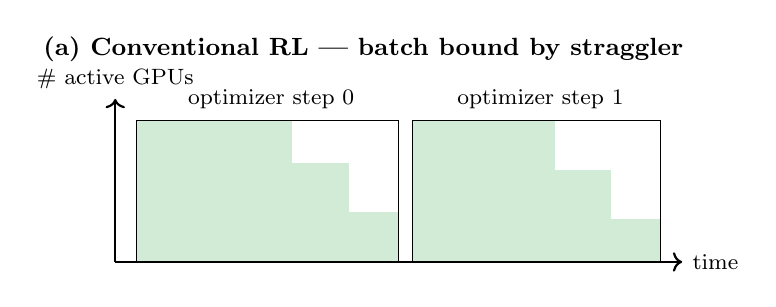
\begin{tikzpicture}[scale=0.9]
  % ---- Conventional RL ----
  \node[font=\small\bfseries] at (3.5, 3) {(a) Conventional RL --- batch bound by straggler};

  \draw[->, thick] (0,0) -- (8,0) node[right, font=\footnotesize] {time};
  \draw[->, thick] (0,0) -- (0,2.3) node[above, font=\footnotesize] {\# active GPUs};

  \fill[inferencegreen] (0.3,0) -- (2.5,0) -- (2.5,2) -- (0.3,2) -- cycle;
  \fill[inferencegreen] (0.3,0) -- (3.3,0) -- (3.3,1.4) -- (0.3,1.4) -- cycle;
  \fill[inferencegreen] (0.3,0) -- (4.0,0) -- (4.0,0.7) -- (0.3,0.7) -- cycle;
  \draw (0.3,0) rectangle (4.0,2);
  \node[font=\footnotesize] at (2.2,2.3) {optimizer step 0};

  \fill[inferencegreen] (4.2,0) -- (6.2,0) -- (6.2,2) -- (4.2,2) -- cycle;
  \fill[inferencegreen] (4.2,0) -- (7.0,0) -- (7.0,1.3) -- (4.2,1.3) -- cycle;
  \fill[inferencegreen] (4.2,0) -- (7.7,0) -- (7.7,0.6) -- (4.2,0.6) -- cycle;
  \draw (4.2,0) rectangle (7.7,2);
  \node[font=\footnotesize] at (6,2.3) {optimizer step 1};
\end{tikzpicture}

\vspace{0.6em}

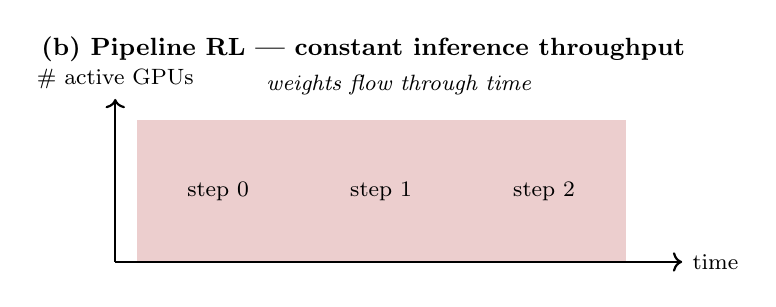
\begin{tikzpicture}[scale=0.9]
  % ---- Pipeline RL ----
  \node[font=\small\bfseries] at (3.5, 3) {(b) Pipeline RL --- constant inference throughput};

  \draw[->, thick] (0,0) -- (8,0) node[right, font=\footnotesize] {time};
  \draw[->, thick] (0,0) -- (0,2.3) node[above, font=\footnotesize] {\# active GPUs};

  \fill[primeaccent!25] (0.3,0) rectangle (2.6,2);
  \fill[primeaccent!25] (2.6,0) rectangle (4.9,2);
  \fill[primeaccent!25] (4.9,0) rectangle (7.2,2);
  \draw (0.3,0) -- (7.5,0);

  \node[font=\footnotesize] at (1.45,1) {step 0};
  \node[font=\footnotesize] at (3.75,1) {step 1};
  \node[font=\footnotesize] at (6.05,1) {step 2};
  \node[font=\footnotesize\itshape] at (4,2.5) {weights flow through time};
\end{tikzpicture}
\end{center}

\subsection{In-Flight Weight Updates}

Pipeline RL dissolves the straggler by dissolving the \emph{batch} as an atomic unit. A single rollout is permitted to span multiple optimizer steps; as new weights are produced by the trainer, they are swapped in mid-flight, and the rollout continues under the updated policy. Inference runs at constant batch size throughout. The longest sequence in the distribution no longer blocks the shortest; each simply contributes its tokens as it produces them, and the advantage is computed using appropriate importance-sampling corrections across whatever policy mixture actually generated the trajectory. Empirically, this can make end-to-end training $3\!\times$ to $5\!\times$ faster as variance in sequence length grows.

% =====================================================================
\section{Agentic RL: Orchestration Under Latency}
% =====================================================================

We now ascend to the regime where the agent does not merely generate text but \emph{interacts}. A rollout in agentic RL alternates between model calls and tool calls --- shell commands, compiler invocations, web searches, sandboxed code executions --- each of which is, from the GPU's perspective, a period of pure idleness.

\begin{center}
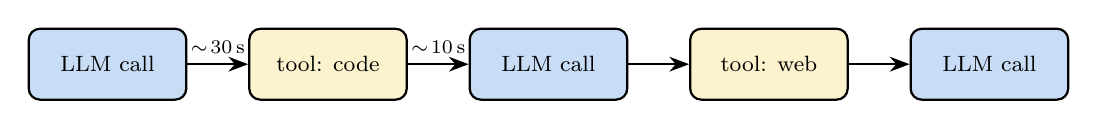
\begin{tikzpicture}[
  stepnode/.style={draw, rounded corners, thick, minimum width=2cm, minimum height=0.9cm, align=center, font=\footnotesize},
  llm/.style={stepnode, fill=trainerblue},
  tool/.style={stepnode, fill=kvyellow},
  arr/.style={-{Stealth[length=2.5mm]}, thick}
]
  \node[llm] (l1) at (0,0) {LLM call};
  \node[tool] (t1) at (2.8,0) {tool: code};
  \node[llm] (l2) at (5.6,0) {LLM call};
  \node[tool] (t2) at (8.4,0) {tool: web};
  \node[llm] (l3) at (11.2,0) {LLM call};

  \draw[arr] (l1) -- node[above, font=\scriptsize]{$\sim\!30\,$s} (t1);
  \draw[arr] (t1) -- node[above, font=\scriptsize]{$\sim\!10\,$s} (l2);
  \draw[arr] (l2) -- (t2);
  \draw[arr] (t2) -- (l3);
\end{tikzpicture}
\end{center}

Empirically, roughly half the wall-clock time of an agentic rollout is spent waiting on tools. A synchronous design leaves inference GPUs idle for that entire duration. The solution is to treat rollouts themselves as asynchronous citizens: when one rollout blocks on a tool call, the inference engine fires ahead on another, maintaining a large pool of in-flight trajectories that collectively keep the GPUs saturated.

\subsection{The Three-Component Architecture}

A production-grade agentic RL stack organizes itself around three cooperating services.

\begin{center}
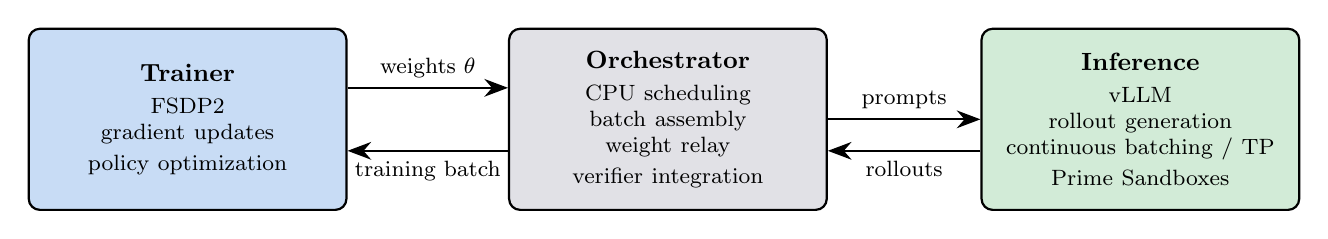
\begin{tikzpicture}[
  mod/.style={draw, rounded corners, thick, minimum width=3.8cm, minimum height=2.3cm, align=center, font=\small, text width=3.8cm},
  arr/.style={-{Stealth[length=3mm]}, thick}
]
  \node[mod, fill=trainerblue] (tr) at (-0.1,0) {\textbf{Trainer}\\[2pt]\footnotesize FSDP2\\gradient updates\\policy optimization};
  \node[mod, fill=orchgray] (or) at (6,0) {\textbf{Orchestrator}\\[2pt]\footnotesize CPU scheduling\\batch assembly\\weight relay\\verifier integration};
  \node[mod, fill=inferencegreen] (in) at (12,0) {\textbf{Inference}\\[2pt]\footnotesize vLLM\\rollout generation\\continuous batching / TP\\Prime Sandboxes};

  \draw[arr] (or) -- node[above, font=\footnotesize] {prompts} (in);
  \draw[arr] ([yshift=-4mm]in.west) -- node[below, font=\footnotesize] {rollouts} ([yshift=-4mm]or.east);

  \draw[arr] ([yshift=4mm]tr.east) -- node[above, font=\footnotesize] {weights $\theta$} ([yshift=4mm]or.west);
  \draw[arr] ([yshift=-4mm]or.west) -- node[below, font=\footnotesize] {training batch} ([yshift=-4mm]tr.east);
\end{tikzpicture}
\end{center}

The \textbf{Trainer} does the mathematics: FSDP2-sharded gradient steps, NCCL broadcasts to synchronize updated weights. The \textbf{Inference} service generates rollouts at high throughput, using vLLM with continuous batching and tensor parallelism, and maintains a fleet of \emph{Prime Sandboxes} for secure, isolated tool execution. Between them sits the \textbf{Orchestrator}: a CPU-bound control plane that schedules prompts, assembles rollout batches, relays weights, integrates verifiers, and --- crucially --- manages the thousands of sandbox instances required to run modern agentic environments.

\begin{remark}
The orchestrator's importance grows superlinearly with agent complexity. For classical RLVR with string-grader math problems, verification is effectively free. For an agent that edits a repository, runs a test suite, and negotiates with a web API, the orchestrator is responsible for spinning up, monitoring, and tearing down actual execution environments --- a Kubernetes-scale concern that has no analog in classical deep learning training.
\end{remark}

\subsection{Oversampling Against Tool Stalls}

Tool calls are not merely slow; they are occasionally \emph{non-terminating}. A model may produce a \texttt{grep} on the filesystem root, a runaway infinite loop, or a request to an unresponsive server. To prevent such trajectories from starving the batch, the system maintains an \emph{oversampling factor}: more rollouts are in flight than any single training batch requires, so that stalled rollouts can be quietly abandoned or timed out without ever leaving the trainer waiting.

% =====================================================================
\section{Long-Horizon RL and Async Pressure}
% =====================================================================

As task horizons lengthen, two things grow together: the variance of a single rollout, and the necessity of async infrastructure to tolerate that variance. The following table, which we shall call the \emph{async-pressure hierarchy}, organizes the regime.

\begin{center}
\renewcommand{\arraystretch}{1.3}
\begin{tabular}{@{}lll@{}}
\toprule
\textbf{Regime} & \textbf{Horizon} & \textbf{Async requirement} \\
\midrule
Single-turn math & $\sim\!1$K tokens & minimal \\
Code generation & $\sim\!10$K tokens & moderate \\
SWE-bench & $\sim\!100$K tokens & substantial \\
Multi-day research & $\sim\!1$M tokens & total decoupling \\
\bottomrule
\end{tabular}
\end{center}

At the top of the hierarchy, a single rollout may involve hours-long experiments --- a scientific agent querying a biological simulation, or a coding agent running a long test campaign. Synchronous RL is not merely inefficient here; it is \emph{impossible}. An on-policy update that waits for each rollout to terminate before taking a gradient step will never make a gradient step at all. Async decoupling ceases to be an optimization and becomes a precondition for learning.

% =====================================================================
\section{State-of-the-Art Inference Infrastructure}\label{sec:inference-infra}
% =====================================================================

In RL, the thing done most often is inference. Three optimizations are, at the time of writing, load-bearing for frontier deployments.

\subsection{Expert Parallelism and Deep-EP}

For MoE models, the number of experts can run into the hundreds, their combined parameter count into the hundreds of billions. Replicating the full expert population on every node is infeasible; we must \emph{partition} experts across GPUs and route tokens dynamically. \textbf{Deep-EP} provides the communication primitives for this routing, avoiding the all-to-all weight replication that would otherwise dominate the cost. At Intellect-3 scale, expert parallelism across 64+ GPUs is not an optimization --- it is the only way the model runs at all.

\subsection{Prefill/Decode Disaggregation}

Inference is two jobs in one uniform. The \textbf{prefill} phase consumes a prompt of $n$ tokens in a single forward pass, is compute-bound, and produces the initial KV cache. The \textbf{decode} phase produces one output token per pass, is memory-bandwidth-bound, and depends critically on low-latency access to a growing KV cache. These phases want different batch shapes, different parallelism strategies, and different GPU SKUs. Running them on separate pools, with a disaggregated KV cache that flows between them, recovers substantial efficiency.

\begin{center}
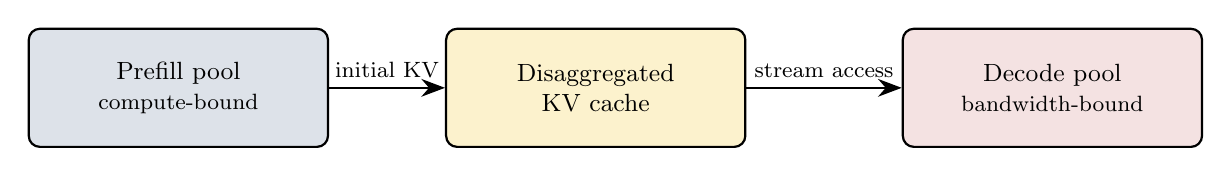
\begin{tikzpicture}[
  pool/.style={draw, rounded corners, thick, minimum width=3.8cm, minimum height=1.5cm, align=center, font=\small},
  arr/.style={-{Stealth[length=3mm]}, thick}
]
  \node[pool, fill=primeblue!15] (pre) at (-0.1,0) {Prefill pool \\ \footnotesize compute-bound};
  \node[pool, fill=kvyellow] (kv) at (5.2,0) {Disaggregated \\ KV cache};
  \node[pool, fill=primeaccent!15] (dec) at (11.0,0) {Decode pool \\ \footnotesize bandwidth-bound};

  \draw[arr] (pre) -- node[above, font=\footnotesize] {initial KV} (kv);
  \draw[arr] (kv) -- node[above, font=\footnotesize] {stream access} (dec);
\end{tikzpicture}
\end{center}

\subsection{NVFP4: Near-Lossless 4-Bit Quantization}

On NVIDIA's Blackwell generation, \textbf{NVFP4} --- a 4-bit floating-point format --- delivers $2\text{--}4\times$ the throughput of FP16 with quality loss typically within $2\text{--}4\%$ of the full-precision model. The practical consequence is dramatic: a 671B-parameter model that would otherwise require a very large cluster can be served on a modest one. Quantization, once a tool of last resort, has become a first-class citizen of the inference stack.

\begin{remark}[The quantization-mismatch recipe]
Fully quantized training at NVF4 is not yet a solved problem. A pragmatic interim is \emph{mixed-precision across phases}: run inference in NVFP4 for throughput, perform training updates in BF16 for numerical stability, and quantize again when transmitting the updated weights back to the inference engine. The resulting train/infer distribution mismatch is one more source of off-policyness, to be absorbed by the same importance-sampling and clipping machinery we have already built.
\end{remark}

% =====================================================================
\section{Prime RL, Verifiers, and the Open Stack}
% =====================================================================

The infrastructure described here is, at Prime Intellect, organized as an open-source stack.

\begin{description}[style=nextline, leftmargin=0.6cm, itemsep=4pt]
  \item[\textbf{Prime RL}.] The open-source RL framework that unifies the above: Deep-EP inference, prefill/decode separation, NVFP4 quantization, pipeline RL with in-flight weight updates. 
  \item[\textbf{Verifier}.] A Python SDK for constructing RL environments: defining problems, designing reward functions, plugging verifiers into the training loop. It is the bridge between a research idea for a new environment and a trainable system.
  \item[\textbf{Environment Hub}.] A shared registry of RL environments --- conceptually, a Hugging Face Hub specialized for tasks, verifiers, and reward functions --- so that environments can be versioned, shared, and tracked.
  \item[\textbf{Prime Lab}.] A hosted platform, built atop Prime RL, that abstracts the underlying infrastructure so that researchers may concentrate on environments and algorithms.

\end{description}

A few points worth underlining, lest they be lost in the technical weeds.

\emph{Off-policyness is a feature, not a bug, once understood.} Asynchronous infrastructure is not an approximation to a ``true'' synchronous ideal; it is what makes long-horizon learning possible. The corrections --- importance sampling, PPO clipping, KL regularization --- are not concessions but the proper mathematical accompaniment of a cluster designed to be always busy.

\emph{Dense and MoE models are not interchangeable.} An MoE model brings parameter efficiency at the cost of routing complexity and a new class of training instabilities. The choice is architectural and must be made early; it ramifies through every layer of the stack.

\emph{The bottleneck migrates.} In 2023 the bottleneck was human labelers. In 2024 it was verifier throughput. In 2025 it is tool-call latency and orchestrator scale. In 2026 --- if the projection holds --- it will be the wall-clock cost of the environments themselves: laboratories, markets, multi-day scientific campaigns. The algorithms and the infrastructure must continue to race ahead of wherever the bottleneck is about to be.

\end{document}